%----------------------------------------------------------------------------------------
%----------------------------------------------------------------------------------------
%----------------------------------------------------------------------------------------
%Method
%----------------------------------------------------------------------------------------
%----------------------------------------------------------------------------------------
%----------------------------------------------------------------------------------------

\section{METHOD}
\label{sec: method}
 \subsection{Self Organizing Maps}
 \label{sec: som}
 
 Kohonen Self organizing map (or self organizing map, SOM) is an unsupervised neural network for mapping and visualizing a complex and non linear high dimension data introduced by~\citep{Kohonen82}. 
 The SOM is a technique that shows a simple geometry relationship of a non-linear high dimension data on a map \citep{Kohonen98}.
 The SOM is a clustering method which reduces the dimension of data to lower dimensions usually 1 or 2D while preserving topological features of the original data.
 Results of SOM contains nodes (usually hexagonal ones) that arranged in 1D or 2D arrays.
 
  
 Each nodes may contain one or more samples from input data and distance between nodes represents similarity or dissimilarity of underlying samples. 
 In the way that similar data are closer together in the array and the further nodes go from each other, the more dissimilarity appears between their samples.
 %Sahar_self_notes: maybe "some" is better instead of one or more
 A weight vector ``\boldit{W}" with same dimension of the input data associates with each node which will be change during the process and has a key factor in a position of nodes in the map. 
 
 \cite{Geach12} presented the application of the SOM and demonstrate the algorithm of the SOM in detail.
 %% Compare SOM with hierarchical methods and PC
 
%  \subsubsection{Algorithm of SOM} 
%  \label{sec: algorithm}
%      Assuming we have a data set which contains vectors, \boldit{V} $\in \Re^n$ and we want to map them on S1 by S2 map. 
%      We start by creating S1 $\times$ S2 empty neurons. 
%      The initial arrangement of these neurons depends on a map's topology provided by user.
%      Since the topology of the map does not have any affect on the final result, we chose hexagonal topology which is the default topology for SOMs.
%      Then, we assign a random weight vector \boldit{W} $\in \Re^n$ to each node.
%      The process of creating SOM, happens over series of $N$ iterations. 
%      During each iteration the weight vectors might change according to the Kohonen learning rule (equation~\ref{equ: weight adj}). 
%       In each iteration:
%      \begin{enumerate}
%         \item Choose a random vector from our data set.
%         \item Calculate the euclidean distance for each node j as  $D_j^2= \sum_{i=0}^{i=n} (V_i - W_i)^2$, and find a neuron with ``$D_{j_{min}}$". This neuron is the winner node and is calling Best Matching Unit (BMU). 
%         \item  Compute the radius of the neighbourhood of the BMU to find nodes within this radius. The weight vectors of these nodes will be affected in the next steps. This value is arbitrary and initially can be set to be as high as half of the SOM size and then it decades exponentially over each iteration:
%         \begin{equation}
%             r^t_{BMU} = r^0_{BMU}e^{(-t/\tau)}
%         \end{equation}
%         where $\tau$ is a decay constant and usually set to be the same as number of iterations, $N$. $r^0_{BMU}$ and $r^t_{BMU}$ is the radius of the neighbourhood at 0th and $t$th iteration, respectively. 
%         \item Change the weight vectors of the BMU and all the nodes within r(t) as:
%         \begin{equation}
%             \label{equ: weight adj}
%             w(t+1)=w(t)+L(t) \times R(t) \times(v(t)-w(t))
%         \end{equation}
%         where $L(t) = L_0 e^{(-t/\tau)}$ is the learning factor which prevents divergence of the SOM and $R(t)=exp(-\frac{D_j^2}{2r^t_{BMU}})$ is the influence rate. $R(t)$ determines how weight of nodes in the neighbourhood of BMU will change.
%         \item  Repeat these steps for $N$ times.
    % \end{enumerate}
     

     In order to create SOM, we used {\tiny MATLAB} neural network toolbox~\citep[NNT,][]{matlabtolbox}.
     SOM in {\tiny NNT} can be created by {\tiny newsom} library which works in two phases; ``ordering phase" and ``tuning phase" . 
     Phase one is the ``ordering phase". 
     This phase starts with maximum neighbourhood distance, and initial high learning factor usually 0.9 which is provided by user. 
     The ordering phase continues for requested number of iterations and it continues till the learning factor reduces to tuning phase leaning factor and the neighbourhood distance reaches to the number set by the user.
     
     The second phase is the ``tuning phase".
     In this phase the neighbourhood distance is at its minimum, but learning factor decreases very slowly.
     This minimum neighbourhood distance and slowly decreasing the leaning factor helps to fine tune the topology results and causes the more stable SOM. 
     The number of iterations in this tuning phase most be much more than the number iterations in ordering phase, to allow the tuning happens slowly. 
     We chose number of epochs the tuning phase be 3 times more than number of epochs in the ordering phase.
     
     
     {\tiny NNT}'s built-in plotting tool plots evolved version of SOMs, which are designed to show distance between each clusters more clear.
     To show the results, we combine two of those plots; a ``Hits map", which shows number of hits for each neurons, and a ``distances map", which shows the same neurons as the hits map and the distance between them. 
     To combine these two maps, in each distance map, we showed wrote the regions that are placed in winner neurons.
     The empty neurons indicate that no region in our sample places in them.
     
     In SOMs, the purple hexagonal shape represent the neurons.
     The distances in a distance map are showing by grey cycle colours between the neurons.
     The white colour represents the high amount of the similarity between neurons, and the darker the colour shows the more differences.
     In Section~\ref{sec: mock_sample} we used {\tiny newsom} to create SOMs from a mock sample to illustrate how this method works and how we can interpret the results.
     
     \subsection{Creating SOM}
    \label{sec: create_som}
     One of the features of clustering methods is that there is no rule and restriction on number of clusters.
     Users usually must decide the size of networks based on their data set and their usages of the results .
     There has been few attempts to find a rule for finding maximum number of neurons based on the input sample \citep[e.g.][]{Vesanto05}, but none of them are certain. 
     We varied size of SOMs from $1\times2$ to $50\times50$ to choose the sufficient size for our maps, and found that based on size of our data the 10$\times$10 in 2D maps are sufficient. 
     
     
     %Also for each grid we created different SOM with different, learning factors, neighbourhood distances, and iteration numbers to find the optimize result for our sample.
     %Based on our data we created our final SOMs with following initial values: number of iteration in ordering phase = 1000; ordering phase learning factor = 0.9; tuning phase learning factor= 0.02; and tuning phase neighbourhood distance to be 1.
     %All the other parameters are default values in {\tiny newsom} library and cannot be changed by the users. 
     
     Some of the correlations between some wavelengths and properties of galaxies are well-known.
     For example, \citep{Rahmani16} used IRAC1 band emission to calculate the stellar mass, or FUV, NUV and MIPS24 emission are used to measure the SFR value. 
     We removed all the observed data, that were used to calculate these properties from the input sample, call the reduce sample the ``subset 0".
     We used the subset 0 sample as the main input of the SOMs, to make sure that we wouldn't use some of the observed data as an input data, in various forms.
     Fig.~\ref{fig: cor_all} shows Pearson correlation coefficients with a confidence level of $95\%$ for all the data in the subset 0 sample.
     
     
     
     
     
     
      \begin{figure}
                \centering
                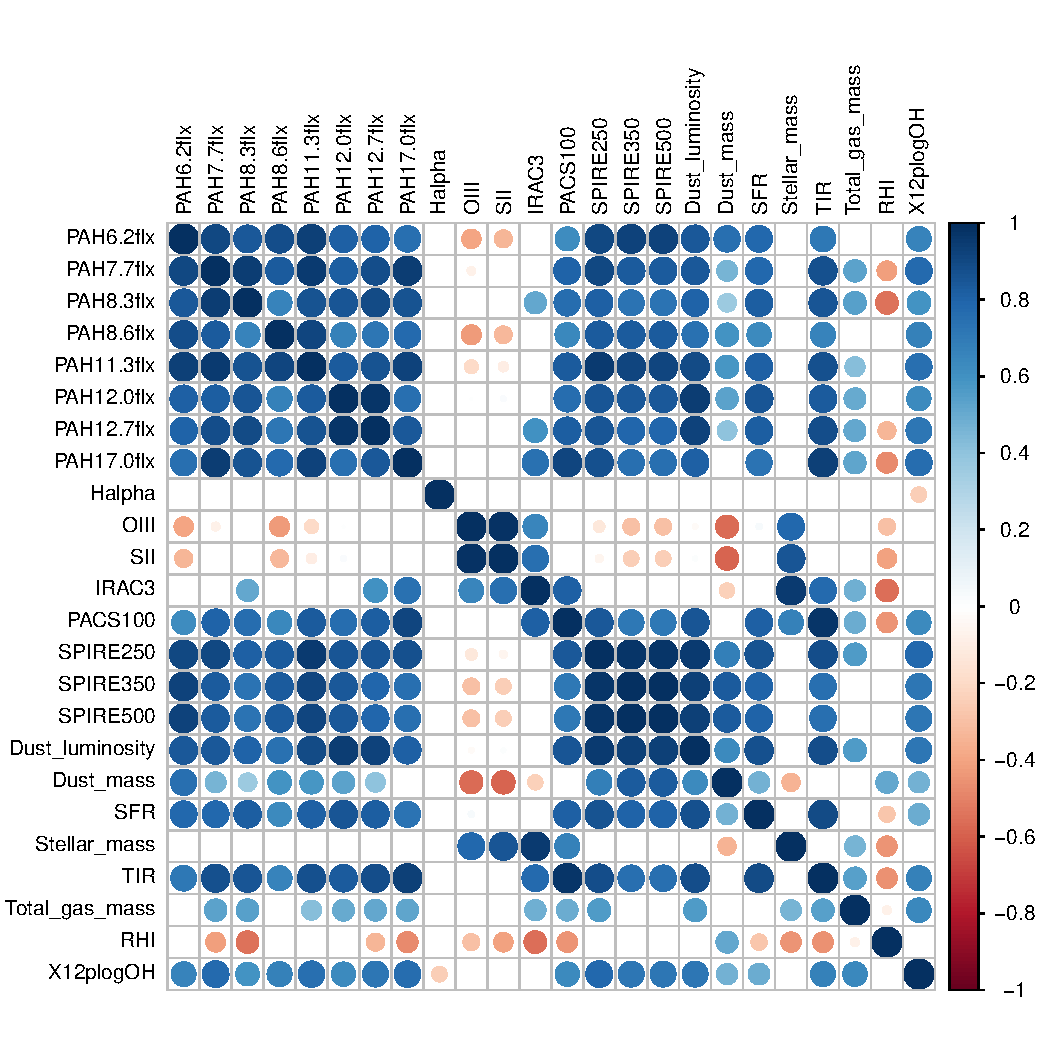
\includegraphics[width=0.5\textwidth]{../images0.01/cor_plots/M31_all_derived_ones_core_plot_for_paper.pdf}
            \caption{Pearson correlation coefficients with a confidence level of 95$\%$ for all the in the subset 0. The colours show the Pearson correlation coefficients where 1 means highly correlated and -1 is highly anti-correlated quantities. The non-significant correlations were left empty.}
            \label{fig: cor_all}
        \end{figure}
 
  
     
    
\subsection{Mock sample}
\label{sec: mock_sample}
 
         \begin{figure}
                \centering
                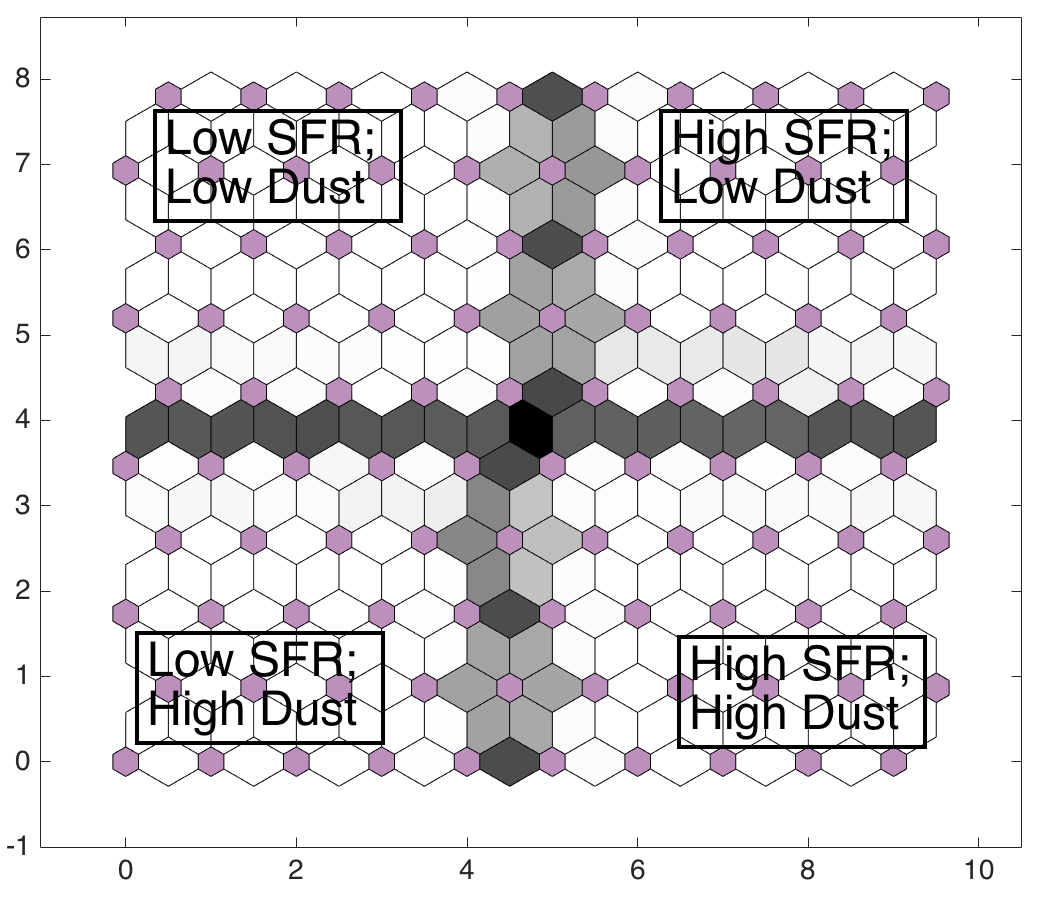
\includegraphics[width=0.5\textwidth]{../images0.01/mock_sample.png}
            \caption{SOM of the mock sample. The axes show the position of the neurons. Hexagonal shapes represent the neurons. The grey cycle colours show the differences between weight of each neuron where white is the minimum differences and black has the maximum one.}
            \label{fig: sample}
        \end{figure}
 
 To make it clear that how this method works, we created a mock sample.
 The mock sample contains a few regions, which we know two information about them; amount of dust and the SFR.
 The input data are so simple and has low dimension; each entry only can get either 0 or 1 as high or low SFR, and 0 or 0.5 as an indicator of high or low amount of dust.
 We generated a SOM with the size of $10 \times 10$ from the sample, using the method that described in Sec.~\ref{sec: method}.
 Fig. ~\ref{fig: sample} shows the SOM of the mock sample. 
 The axes show the position of the neurons in a $10 \times 10$ network and the hexagonal shapes are the neurons.
 
 
Using this method, as we could predict, we were able to divide the mock sample's regions into 4 distinct groups: regions with high SFR and high amount of dust, regions with low SFR and high amount of dust, regions with high SFR and low amount of dust, and regions low SFR and low amount of dust. 
The plot in the Fig.~\ref{fig: sample}, clearly shows these divisions.
In that plot, the upper part belongs to regions with low amount of dust, while the lower part belongs to the high amount of dust.
The left part of the plot, is where regions with low SFR belong to and the right side is for high SFR regions.
Grey to black colours show the border between regions.
This network is considered as a trained network, and can used to cluster any new data set with similar entries.

Having two regions with exactly the same values in all their quantities is almost impossible. 
Therefore, one can find a network with high amount of the neurons, which separates the input data completely, and clusters them into separate groups.
However, if the input data are very similar to one another, such a network must have much higher number of the neurons than the number of input samples. 
Based on the relative size of the network to the input data, the users can learn about the similarity/dissimilarity among input quantities.

